\chapter{Newton's Laws and Free-Body Diagrams}
\label{ch:newton}
\begin{chapterintro}
\textbf{You will learn to:} state Newton's three laws; draw a correct free-body
diagram; write the equations of motion along convenient axes; and solve
equilibrium and circular-motion problems.
\end{chapterintro}

\section{Newton's laws}

\begin{enumerate}[leftmargin=1.7em,itemsep=4pt]
  \item \textbf{Inertia.} In an inertial frame, a body remains at rest or in
        uniform rectilinear motion unless acted on by a net external force.
  \item \textbf{Fundamental principle of dynamics.}
        \[
        \sum\vec F_{\text{ext}}
        =\frac{\dd\vec p}{\dd t}
        =\frac{\dd(m\vec v)}{\dd t}.
        \]
        For constant mass,
        \[
        \boxed{\sum\vec F_{\text{ext}}=m\vec a.}
        \]
  \item \textbf{Action--reaction.} If $A$ exerts a force on $B$, then $B$ exerts
        on $A$ a force equal in magnitude and opposite in direction:
        \[
        \vec F_{B\to A}=-\vec F_{A\to B}.
        \]
\end{enumerate}

The three laws are valid in an \textbf{inertial frame}. A frame accelerating or
rotating relative to an inertial frame requires the fictitious forces of
\cref{ch:relative}.

\section{Standard force models}

\begin{center}
\renewcommand{\arraystretch}{1.3}
\begin{tabular}{@{}p{0.22\textwidth}p{0.34\textwidth}p{0.36\textwidth}@{}}
\toprule
\textbf{Force} & \textbf{Expression} & \textbf{Direction} \\
\midrule
Weight & $\vec W=m\vec g$ & vertical, downward \\
Normal reaction & $\vec N$ & perpendicular to the surface, away from it \\
Tension & $T$ & along the string, pulling the body \\
Spring (Hooke) & $\vec F=-k(l-l_0)\vec u$ & toward the equilibrium position \\
Solid friction & $f\le\mu_sN$, $f_k=\mu_kN$ & opposite to the tendency of sliding \\
Viscous drag & $\vec f=-k\vec v$ & opposite to the velocity \\
Universal gravity & $\vec F=-GMm\,\ur/r^2$ & attractive, toward the other mass \\
\bottomrule
\end{tabular}
\end{center}

\begin{figure}[htbp]
\centering
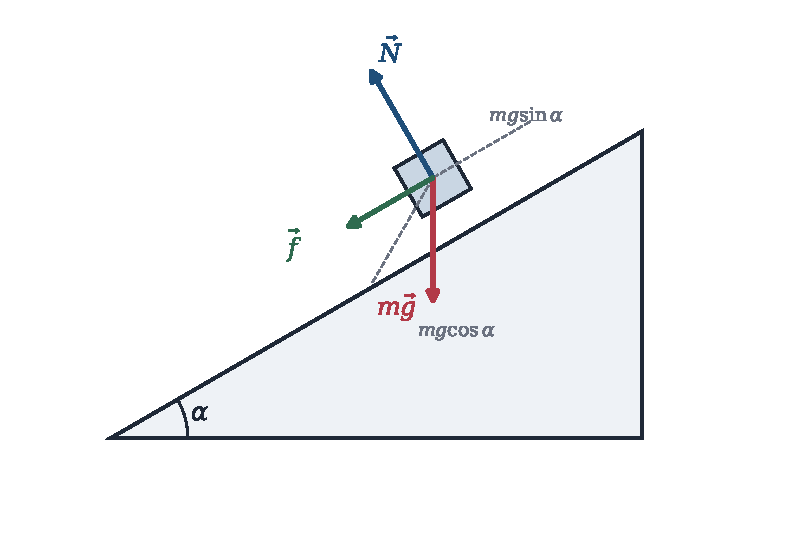
\includegraphics[width=0.82\textwidth]{figures/11_incline_fbd.pdf}
\caption{Free-body diagram for a block on an inclined plane. The weight is
decomposed into components parallel and perpendicular to the plane.}
\label{fig:incline-fbd}
\end{figure}

\section{The free-body diagram method}

\begin{method}[Five steps that solve most problems]
\begin{enumerate}[leftmargin=1.6em,itemsep=2pt]
  \item Isolate the body of interest.
  \item Draw every external force acting \emph{on} it (not forces it exerts on
        other bodies).
  \item Choose axes: along the motion and perpendicular to it.
  \item Decompose the forces along the axes.
  \item Apply $\sum F_x=ma_x$, $\sum F_y=ma_y$. If the body does not accelerate
        in a direction, the sum of forces in that direction is zero.
\end{enumerate}
\end{method}

\begin{warning}[Two classic errors]
Do not put both the weight $m\vec g$ and its components $mg\sin\alpha$,
$mg\cos\alpha$ on the same diagram: choose one representation. Do not include
the force that the body exerts on something else; the diagram is only about
forces \emph{on} the body.
\end{warning}

\section{Dynamics of circular motion}

For a particle moving on a circle of radius $R$, project Newton's second law on
the inward radial direction and on the tangent:
\[
\sum F_{\text{radial}}=m\frac{v^2}{R},
\qquad
\sum F_{\text{tangential}}=m\frac{\dd v}{\dd t}.
\]
The radial equation is not a new law; it is $m\vec a$ written in the normal and
tangential directions.

% ===========================================================================
\section{Worked examples}

\begin{worked}[Block on a frictionless incline]
A block of mass $m=5.00\ \mathrm{kg}$ rests on a frictionless plane inclined at
$\alpha=30.0^\circ$. Find its acceleration and the normal reaction.
\end{worked}

\begin{solution}{8.1}
Take axes parallel and perpendicular to the plane. The only forces are the weight
$m\vec g$ and the normal $\vec N$. The weight components are
$mg\sin\alpha$ down the slope and $mg\cos\alpha$ into the plane.

Perpendicular to the plane there is no acceleration:
\[
N-mg\cos\alpha=0
\implies
N=mg\cos\alpha.
\]
Parallel to the plane:
\[
mg\sin\alpha=ma
\implies
a=g\sin\alpha.
\]
Numerically,
\[
a=9.81\sin30.0^\circ=4.91\ \mathrm{m\,s^{-2}},
\]
\[
N=5.00(9.81)\cos30.0^\circ=42.5\ \mathrm{N}.
\]
\end{solution}

\begin{worked}[Apparent weight in an elevator]
A person of mass $m=70.0\ \mathrm{kg}$ stands on a scale in an elevator. Find the
scale reading when the elevator (a) is at rest, (b) accelerates upward at
$2.00\ \mathrm{m\,s^{-2}}$, (c) accelerates downward at $2.00\ \mathrm{m\,s^{-2}}$,
and (d) is in free fall.
\end{worked}

\begin{solution}{8.2}
The scale reads the normal force $N$. Take upward as positive. Newton's second
law:
\[
N-mg=ma
\implies
N=m(g+a).
\]
(a) $a=0$:
\[
N=70.0(9.81)=687\ \mathrm{N}.
\]
(b) $a=+2.00\ \mathrm{m\,s^{-2}}$:
\[
N=70.0(9.81+2.00)=827\ \mathrm{N}.
\]
(c) $a=-2.00\ \mathrm{m\,s^{-2}}$:
\[
N=70.0(9.81-2.00)=547\ \mathrm{N}.
\]
(d) $a=-g$:
\[
N=70.0(9.81-9.81)=0.
\]
The person feels weightless.
\end{solution}

% ===========================================================================
\section{Exercises and Step-by-Step Solutions}

\begin{exercise}{\warm\ Newton's second law}
A net force of $30.0\ \mathrm{N}$ acts on a $10.0\ \mathrm{kg}$ body initially at
rest. Find its acceleration, its speed after $4.00\ \mathrm{s}$, and the distance
travelled.
\end{exercise}

\begin{tabletworkspace}[6.5cm]
\end{tabletworkspace}

\begin{solution}{8.1}
\[
a=\frac Fm=\frac{30.0}{10.0}=3.00\ \mathrm{m\,s^{-2}}.
\]
\[
v=at=3.00(4.00)=12.0\ \mathrm{m\,s^{-1}}.
\]
\[
d=\frac12at^2=\frac12(3.00)(4.00)^2=24.0\ \mathrm{m}.
\]
\end{solution}

\begin{exercise}{\warm\ Mass and weight}
A $60.0\ \mathrm{kg}$ astronaut travels to the Moon, where
$g_{\text{Moon}}=1.62\ \mathrm{m\,s^{-2}}$. Find her mass and weight on Earth and
on the Moon.
\end{exercise}

\begin{tabletworkspace}[6.5cm]
\end{tabletworkspace}

\begin{solution}{8.2}
Mass is an intrinsic property, so $m=60.0\ \mathrm{kg}$ everywhere.

On Earth:
\[
W_E=mg_E=60.0(9.81)=589\ \mathrm{N}.
\]
On the Moon:
\[
W_M=mg_M=60.0(1.62)=97.2\ \mathrm{N}.
\]
\end{solution}

\begin{exercise}{\warm\ Elevator scale}
A $75.0\ \mathrm{kg}$ person stands on a scale in an elevator. Find the reading
when the elevator (a) is at rest, (b) accelerates upward at
$2.00\ \mathrm{m\,s^{-2}}$, (c) accelerates downward at $2.00\ \mathrm{m\,s^{-2}}$,
and (d) is in free fall.
\end{exercise}

\begin{tabletworkspace}[6.5cm]
\end{tabletworkspace}

\begin{solution}{8.3}
With upward positive, $N-mg=ma$, so $N=m(g+a)$.

(a) $N=75.0(9.81)=736\ \mathrm{N}$.

(b) $N=75.0(9.81+2.00)=886\ \mathrm{N}$.

(c) $N=75.0(9.81-2.00)=586\ \mathrm{N}$.

(d) $N=0$.
\end{solution}

\begin{exercise}{\core\ Sliding down an incline}
A block of mass $8.00\ \mathrm{kg}$ slides from rest down a frictionless incline
of angle $25.0^\circ$. Find its acceleration, the normal reaction, and the time
to slide $10.0\ \mathrm{m}$.
\end{exercise}

\begin{tabletworkspace}[6.5cm]
\end{tabletworkspace}

\begin{solution}{8.4}
\[
a=g\sin25.0^\circ=9.81(0.4226)=4.15\ \mathrm{m\,s^{-2}}.
\]
\[
N=mg\cos25.0^\circ=8.00(9.81)(0.9063)=71.1\ \mathrm{N}.
\]
From $s=\frac12at^2$,
\[
t=\sqrt{\frac{2s}{a}}=\sqrt{\frac{20.0}{4.15}}=2.20\ \mathrm{s}.
\]
\end{solution}

\begin{exercise}{\core\ Atwood machine}
Two masses $m_1=3.00\ \mathrm{kg}$ and $m_2=5.00\ \mathrm{kg}$ hang from a
massless string over a frictionless pulley. Find the acceleration of the masses
and the tension in the string.
\end{exercise}

\begin{tabletworkspace}[6.5cm]
\end{tabletworkspace}

\begin{solution}{8.5}
Let $a$ be the acceleration of $m_2$ downward (and of $m_1$ upward). For $m_2$:
\[
m_2g-T=m_2a.
\]
For $m_1$:
\[
T-m_1g=m_1a.
\]
Adding,
\[
(m_2-m_1)g=(m_1+m_2)a,
\]
\[
a=\frac{(5.00-3.00)(9.81)}{8.00}=2.45\ \mathrm{m\,s^{-2}}.
\]
Then
\[
T=m_1(g+a)=3.00(9.81+2.45)=36.8\ \mathrm{N}.
\]
\end{solution}

\begin{exercise}{\core\ Two blocks in contact}
A horizontal force $F=20.0\ \mathrm{N}$ pushes a block $m_1=2.00\ \mathrm{kg}$
which is in contact with a block $m_2=3.00\ \mathrm{kg}$ on a frictionless
horizontal surface. Find the acceleration and the contact force between the
blocks. What is the contact force if the force is applied to $m_2$ instead?
\end{exercise}

\begin{tabletworkspace}[6.5cm]
\end{tabletworkspace}

\begin{solution}{8.6}
The two blocks move together:
\[
a=\frac{F}{m_1+m_2}=\frac{20.0}{5.00}=4.00\ \mathrm{m\,s^{-2}}.
\]
For $m_2$, the only horizontal force is the contact force $N_c$:
\[
N_c=m_2a=3.00(4.00)=12.0\ \mathrm{N}.
\]
If the force is applied to $m_2$, the contact force acts on $m_1$:
\[
N_c'=m_1a=2.00(4.00)=8.00\ \mathrm{N}.
\]
\end{solution}

\begin{exercise}{\core\ Car on a flat curve}
A car rounds a flat curve of radius $50.0\ \mathrm{m}$. The coefficient of static
friction between the tyres and the road is $\mu_s=0.600$. Find the maximum speed
before skidding.
\end{exercise}

\begin{tabletworkspace}[6.5cm]
\end{tabletworkspace}

\begin{solution}{8.7}
The static friction provides the centripetal force:
\[
f_s=m\frac{v^2}{R}.
\]
At the limit $f_s=\mu_sN=\mu_smg$, so
\[
\mu_smg=m\frac{v_{\max}^2}{R}
\implies
v_{\max}=\sqrt{\mu_sgR}.
\]
\[
v_{\max}=\sqrt{(0.600)(9.81)(50.0)}=\sqrt{294}=17.2\ \mathrm{m\,s^{-1}}.
\]
\end{solution}

\begin{exercise}{\core\ Conical pendulum}
A ball of mass $0.500\ \mathrm{kg}$ is attached to a string of length
$1.00\ \mathrm{m}$ and moves in a horizontal circle, the string making
$30.0^\circ$ with the vertical. Find the tension and the speed of the ball.
\end{exercise}

\begin{tabletworkspace}[6.5cm]
\end{tabletworkspace}

\begin{solution}{8.8}
Let $\theta=30.0^\circ$ and let $r=L\sin\theta$ be the radius of the circle.
Vertical equilibrium:
\[
T\cos\theta=mg
\implies
T=\frac{mg}{\cos\theta}.
\]
Horizontal (radial) equation:
\[
T\sin\theta=m\frac{v^2}{r}.
\]
Substituting $T$ and $r$:
\[
mg\tan\theta=m\frac{v^2}{L\sin\theta}
\implies
v^2=gL\sin\theta\tan\theta.
\]
Numerically,
\[
T=\frac{0.500(9.81)}{\cos30.0^\circ}=5.66\ \mathrm{N},
\]
\[
v=\sqrt{9.81(1.00)\sin30.0^\circ\tan30.0^\circ}
=\sqrt{2.83}=1.68\ \mathrm{m\,s^{-1}}.
\]
\end{solution}

\begin{exercise}{\core\ Table and hanging mass}
A block $m_1=4.00\ \mathrm{kg}$ on a frictionless horizontal table is connected
by a string over a pulley to a hanging mass $m_2=2.00\ \mathrm{kg}$. Find the
acceleration and the tension.
\end{exercise}

\begin{tabletworkspace}[6.5cm]
\end{tabletworkspace}

\begin{solution}{8.9}
For the hanging mass:
\[
m_2g-T=m_2a.
\]
For the block on the table:
\[
T=m_1a.
\]
Adding,
\[
m_2g=(m_1+m_2)a
\implies
a=\frac{2.00(9.81)}{6.00}=3.27\ \mathrm{m\,s^{-2}}.
\]
\[
T=m_1a=4.00(3.27)=13.1\ \mathrm{N}.
\]
\end{solution}

\begin{exercise}{\mastery\ Time-dependent force}
A body of mass $m$ starts from rest under a force
$F(t)=F_0(1-t/T)$ along a straight line, where $F_0$ and $T$ are positive
constants. Find $v(t)$ and $x(t)$. Find the speed and position at $t=T$, and
describe the motion for $t>T$.
\end{exercise}

\begin{tabletworkspace}[6.5cm]
\end{tabletworkspace}

\begin{solution}{8.10}
\[
a(t)=\frac{F(t)}{m}=\frac{F_0}{m}\left(1-\frac tT\right).
\]
Integrating with $v(0)=0$:
\[
v(t)=\frac{F_0}{m}\left(t-\frac{t^2}{2T}\right).
\]
Integrating again with $x(0)=0$:
\[
x(t)=\frac{F_0}{m}\left(\frac{t^2}{2}-\frac{t^3}{6T}\right).
\]
At $t=T$:
\[
v(T)=\frac{F_0}{m}\left(T-\frac T2\right)=\frac{F_0T}{2m},
\]
\[
x(T)=\frac{F_0}{m}\left(\frac{T^2}{2}-\frac{T^2}{6}\right)
=\frac{F_0T^2}{3m}.
\]
For $t>T$ the force becomes negative: the body decelerates, reverses direction
after stopping, and then accelerates in the opposite direction.
\end{solution}

\begin{exercise}{\mastery\ Vertical loop}
A small block of mass $m$ slides inside a vertical circular loop of radius $R$.
At the top of the loop, find the minimum speed for which it remains in contact
with the track. If its speed at the top is $\sqrt{2gR}$, find the normal force
there.
\end{exercise}

\begin{tabletworkspace}[6.5cm]
\end{tabletworkspace}

\begin{solution}{8.11}
At the top of the loop, both the weight and the normal force point downward
(toward the centre):
\[
N+mg=m\frac{v^2}{R}.
\]
The block remains in contact as long as $N\ge0$, so
\[
m\frac{v^2}{R}\ge mg
\implies
v\ge\sqrt{gR}.
\]
Thus $v_{\min}=\sqrt{gR}$.

If $v=\sqrt{2gR}$,
\[
N=m\frac{2gR}{R}-mg=2mg-mg=mg.
\]
\end{solution}

